\documentclass{standalone}

% Preamble
\begin{document}

\subsection{Numerical experiment}
We provide a reproducible computational experiment that illustrates the effectiveness of the method presented in this article. To perform the computations, follow the steps mentioned in the README.md file of the git repository \cite{jp_code}.
In this experiment, we solve the polynomial system $f = [\\ 
\input{txt/P.txt}$]\\
The size of the Bezout matrix $B^{(0)}$ is $\input{txt/Dx.txt}$; this is the maximum number of solutions that a system of degree \input{txt/deg.txt} can have. To initiate the reduction process, the rank of $B^{(0)}$ is needed; as the matrix has integer coefficients, we use the Sage function matrix.kernel() to calculate its rank. After the reduction process has been completed, we find that the dimension of the quotient $A$ is $\input{txt/bezout_exact_dim.txt}$. The Bezout matrices have rational entries as well as the companion matrices $X_j = B^{(j)}{B^{(0)}}^{-1}$ ; computing the numerical eigenvalues of the $X_j$'s give approximations of the roots of the polynomial system~$f$.

\subsection{Testing the result}
We test the result of the calculations by two means. 
\begin{itemize}
\item[-]
First, we compare the dimension of the quotient $A$, as provided by the Groebner basis, to the dimension provided by the Bezout process, i.e the size of the reduced Bezout matrices. If, as it is the case in this experiment, the polynomial system is in complete intersection, then the two dimensions coincide. If, on the contrary, the polynomial system is not in complete intersection, then the dimension provided by the Groebner basis is infinite whereas the dimension provided by the Bezout process is always finite.
\item[-]
Secondly, we check that $f(X) = 0$, i.e $f_i(X_1,\cdots, X_n) = 0$ for every $i = 1\cdots, n$ and where the $X_j$'s are the companion matrices. When the polynomial system is in complete intersection, this means that every $f_i$ belongs to the ideal $\langle f\rangle$. But, in practice, since the companion matrices have rational entries, the calculation of each $f_i(X_1,\cdots, X_n)$ may be too heavy. Rather, we choose to make the computations in a finite field $F$, typically $\mathbb{Z}/ p\mathbb{Z}$ with, in this experiment, $p = 2003$. Moreover, to lighten even more the computation, we choose a random vector $v\in F$ and compute only the product of each $f_i(X_1,\cdots, X_n)$ by $v$. Thus, we only need to do matrix-vector products. If at the end of the process, and for all $i= 1\cdots, n$, we have $f_i(X_1,\cdots, X_n)v = 0$ then we can conclude that, with a very high probability, $f(X) = 0$. In this experiment we know that the test was succesful because in the sage variable test_XX (a Python list) all the entries equal True.
\end{itemize}

\subsubsection{Quality of the results}
To check the quality of the numerical roots $\alpha$, we compute the errors $Df(\alpha)^{-1}f(\alpha)$.
Table \ref{tab:histo} shows these errors.
\begin{table}[h]
\begin{center}
\begin{tabular}{c|c}
 log10 of errors & nb of roots \\ 
 \hline
 \input{txt/histogram.txt}
\end{tabular}
\end{center}
\caption{histogram of errors}
\label{tab:histo}
\end{table}

\subsubsection{Timings}
Table \ref{tab:timings} shows the timings of the Bezout computations as compared to the timings of the Groebner computations.
\begin{table}[h]
\begin{center}
\begin{tabular}{llllr}
 Method & Computation & Software & Arithmetic & Timing \\ \hline
   \multirow{4}{*}{Bezout} & Bezout matrices & NumPy & floating point & $\input{txt/construction_B_time.txt}$ s \\
   & rank of $B(1)$ via rref()  & Sage & integer & $\input{txt/rank_B0_time.txt}$ s \\
   & reduction process & Sage & integer & $\input{txt/reductions_time.txt}$ s \\
   & eigenvalues & SciPy & floating point & $\input{txt/compute_roots_time.txt}$ s \\ 
   \hline
   \hline
   Groebner & Groebner basis & Sage & integer & $\input{txt/grobner_time.txt}$ s
\end{tabular}
\end{center}
\caption{timings}
\label{tab:timings}
\end{table}

\subsubsection{Size of output}
Table \ref{tab:sizes} shows the disk space used by the Bezout matrices (after the reduction process; only the non-zero entries are taken in account) as compared to the disk space used by the Groebner basis.
\begin{table}[h]
\begin{center}
\begin{tabular}{llc}
 Method & Output & Disk space usage \\ \hline
   \multirow{2}{*}{Bezout} & reduced Bezout matrices & $\input{txt/bezout_size.txt}$ Mo\\
   & (non-zero entries only) & \\
   \hline
   \hline
   Groebner & Groebner basis & $\input{txt/grobner_size.txt}$ Mo
\end{tabular}
\end{center}
\caption{sizes}
\label{tab:sizes}
\end{table}



\end{document}


\iffalse
an histogram (Figure \ref{fig:roots}).
\begin{figure}[p]
    \caption{Histogram of errors}
  \label{fig:roots}
  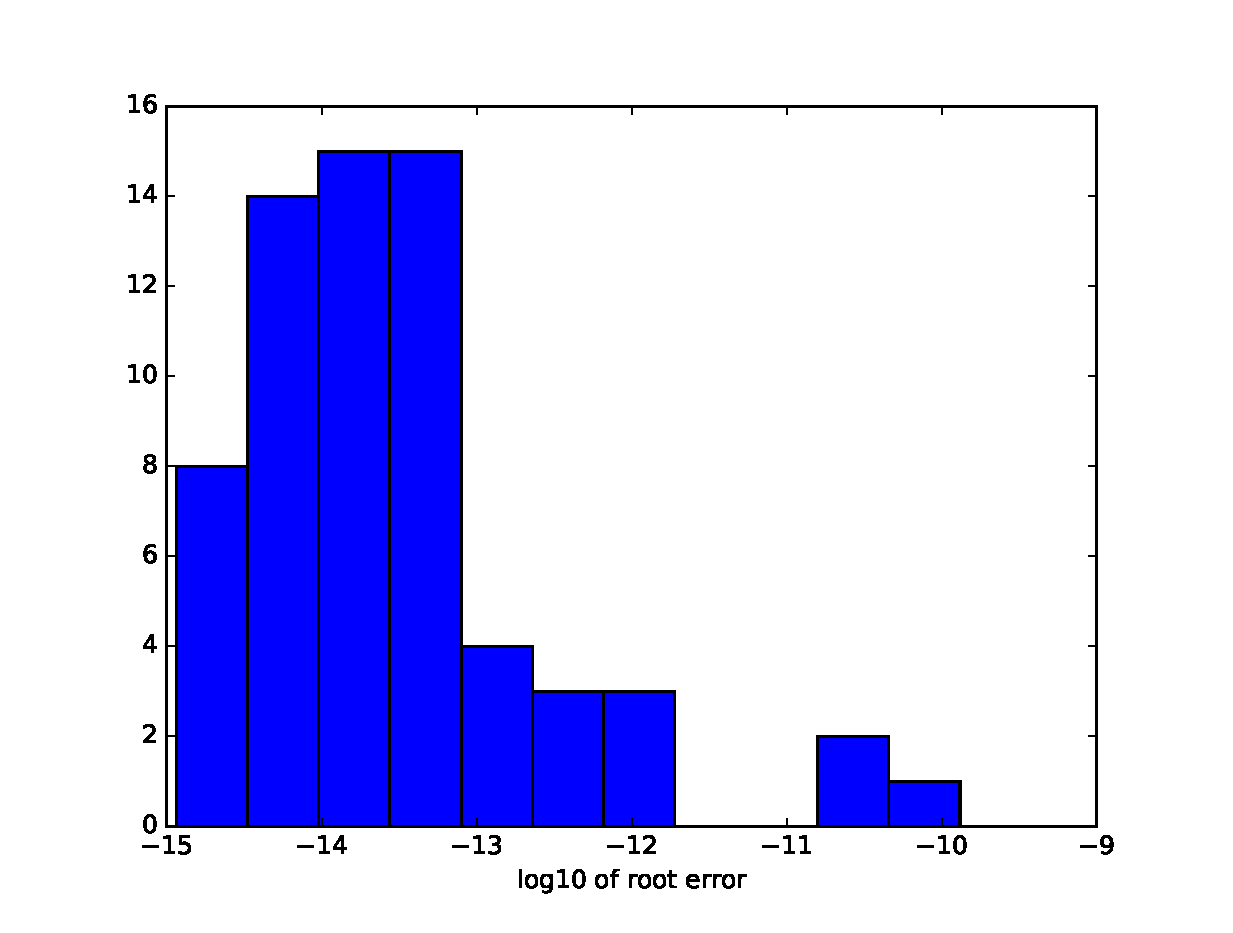
\includegraphics[scale=0.5]{txt/histo_roots.eps}
\end{figure}
\fi
